\subsection{Andamento dei coefficienti di Fresnel}\label{subsec:analisi-coefficienti}
  I dati raccolti sono riassunti in Fig.\ref{fig:dati-raw}.
  Le miglior stime dei parametri, risultato dei \emph{fit}, sono riassunte in Tab.\ref{tab:risultati-fit}
  assieme agli errori standard associati.
  I \emph{fit} sono stati svolti usando l'algoritmo \emph{Gradient}\footnote{https://reference.wolfram.com/language/ref/NonlinearModelFit.html} di \emph{Woflram Mathematica}\footnote{https://www.wolfram.com/mathematica/}.
  Qualitativamente, l'andamento è concorde con quanto atteso. In Fig.\ref{fig:raw-pi}
  si vede chiaramente che la funzione raggiunge lo zero per un certo valore di $\theta$,
  mentre in Fig.\ref{fig:raw-sigma} la funzione cresce monotonamente.
  I residui sono contenuti quasi completamente entro le barre di errore.
  % todo add barre di errore nel grafico dei residui
  %
  \begin{figure}[H]
    \centering
    \begin{subfigure}[t]{.47\textwidth}
      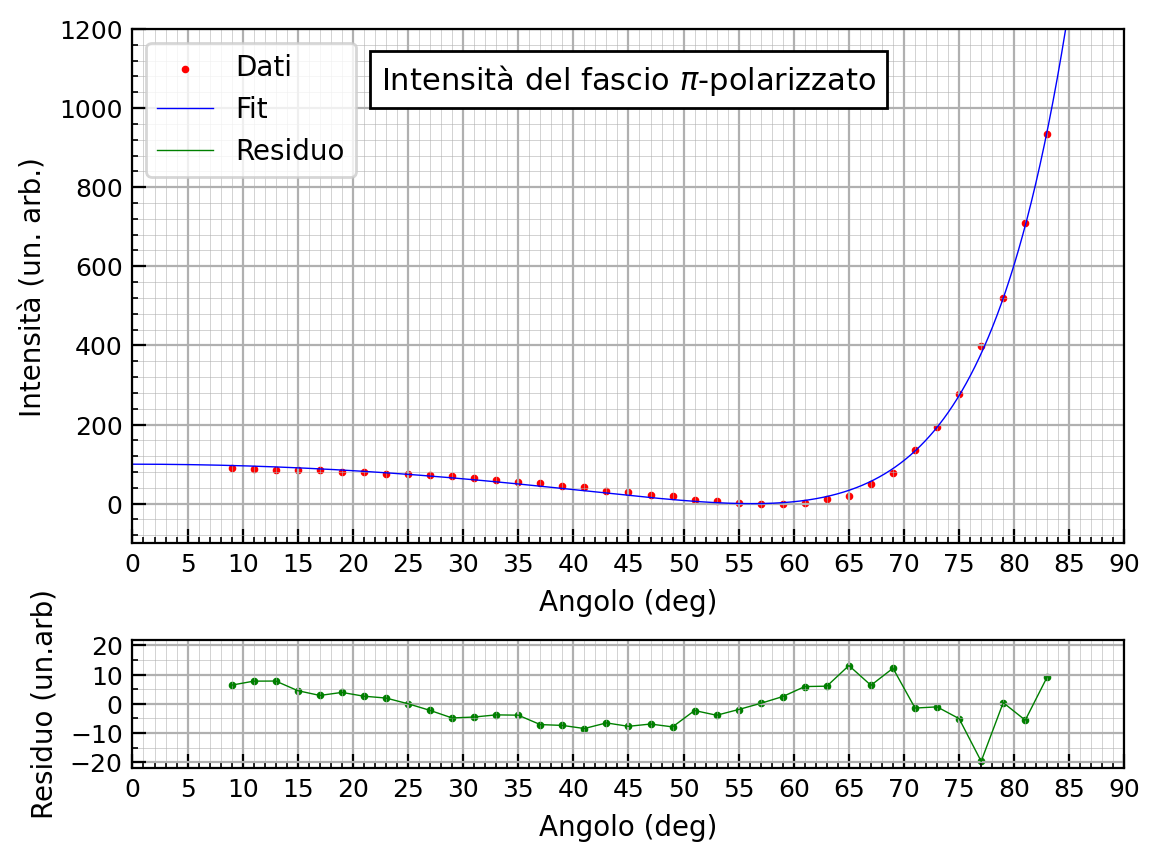
\includegraphics[width=7cm]{./graphs/raw-pi.png}
      \caption{
        \emph{
          Dati di intensità luminosa con luce polarizzata perpendicolarmente al
          piano di incidenza e relativo fit. Dal grafico si vede chiaramente che
          l'intensità luminosa si annulla per un certo valore di $\theta_i$.
        }
      }
      \label{fig:raw-pi}
    \end{subfigure}
    %
    \hspace{5mm}
    %
    \begin{subfigure}[t]{.47\textwidth}
      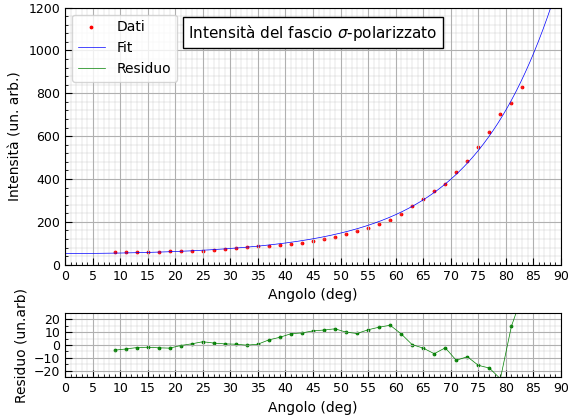
\includegraphics[width=7cm]{./graphs/raw-sigma.png}
      \caption{
        \emph{
          Dati di intensità luminosa con luce polarizzata parallelamente al
          piano di incidenza e relativo fit.
        }
      }
      \label{fig:raw-sigma}
    \end{subfigure}
    \caption{\emph{Dati raccolti.}
    \label{fig:dati-raw}}
  \end{figure}
  %
  \begin{table}[H]
    \centering
    \begin{tabular}[t]{cc}
      \toprule
      Parametro &Valore ottenuto\\
      \midrule
      $I_{0\pi}$ &$2550 \pm 10 (un. arb.)$ \\
      $I_{0\sigma}$ &$1350 \pm 20 (un. arb.)$ \\
      $n_{2\pi}$ &$1.493 \pm 0.006$    \\
      $n_{2\sigma}$ &$1.490 \pm 0.010$    \\
      $\tilde \chi^2_\pi$ &$0.71$ \\
      $\tilde \chi^2_\sigma$ &$1.17$ \\
      \bottomrule
      \end{tabular}
    \caption{
      Risultati dei \emph{fit} dei dati raccolti. Le intensità sono espresse in unità arbitrare, gli indici
      di rifrazione e i chi quadro ridotti sono numeri puri.
    }
    \label{tab:risultati-fit}
  \end{table}
  %
  Abbiamo misurato valori in un intervallo ${\theta_{min} \leq \theta \leq \theta_{max}}$,
  con ${\theta_{min} = 7^\circ \pm 0.5^\circ}$ e $\theta_{max} = 83^\circ \pm 0.5^\circ$.
  Le dimensioni del lato del prisma utilizzato ($15mm$) non permettevano
  di andare oltre $\theta_{max}$ senza che il fascio venisse alterato, mentre il
  limite di $\theta_{min}$ ci è stato imposto dalla geometria del sensore.
  Abbiamo usato un passo angolare di $2^\circ$ per permetterci di prendere un
  numero adeguato di misure, senza allungare eccessivamente la durata dell'esperimento.
  Il campione di dati riportato in Fig.\ref{fig:dati-raw} è quello che segue meglio
  l'andamento previsto.
  Le incertezze associate ad ogni punto sono state ottenute come somma di:
  (incertezze sistematiche dovute all'attrezzatura) $+$ (incertezze casuali), calcolate come
  descritto in Sez.\ref{subsec:calcolo-incertezza-strumentale} e Sez.\ref{subsec:calcolo-incertezza-casuale}. L'incertezza di $\pm 0.5^\circ$ del servomotore
  è da considerarsi già inclusa nelle incertezze sistematiche.
  Normalizzando i dati (dividendo i valori misurati per il parametro $I_0$ del \emph{fit}), si ottengono i risultati mostrati in Fig.\ref{fig:normalised-coefficients}
  % per normalizzare basta dividere per I_0, o conviene imporre anche che i due n2 siano uguali?
  % ceh in realtà ci sta prenderne la media per soddisfare a condizione descritta in Lipson.
  % noi non l'abbiamo fatto.
  assieme all'andamento previsto\footnote{Calcolato supponendo di avere un valore di $1.50 \leq n_2 \leq 1.53$,
  caratteristico per il vetro K9 alla lunghezza della luce rossa.}. % abbiamo anche aggiunto un range I_0 del 10%. è per far venire meglio il grafico.
  %
  \begin{figure}[H]
    \centering
    \begin{subfigure}[t]{.47\textwidth}
      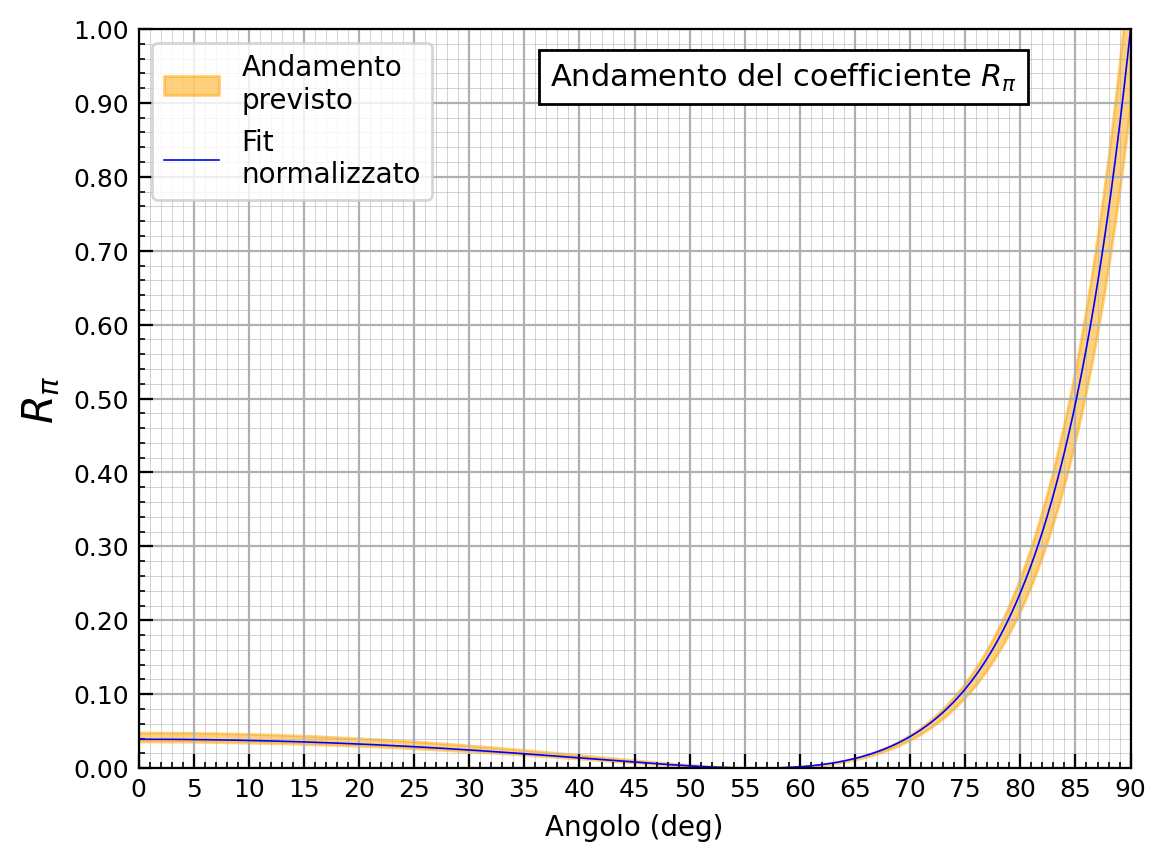
\includegraphics[width=7cm]{./graphs/r-pi-coefficient.png}
      \caption{
        \emph{
          Andamento del coefficiente $R_\pi$, ottenuto normalizzando i dati
          di Fig.\ref{fig:raw-pi}
        }
      }
      \label{fig:normalised-coefficients}
    \end{subfigure}
    %
    \hspace{5mm}
    %
    \begin{subfigure}[t]{.47\textwidth}
      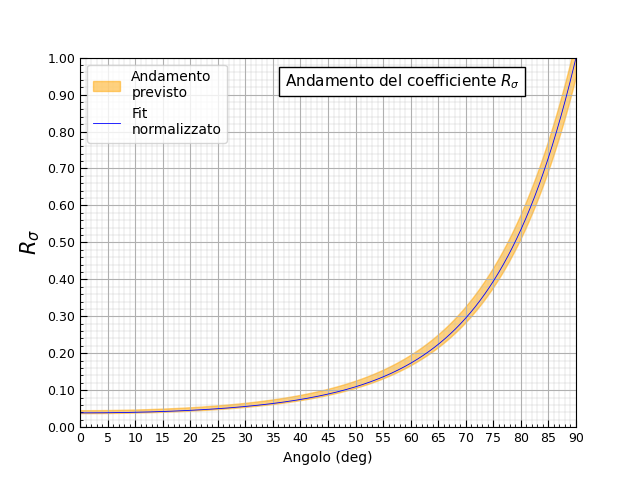
\includegraphics[width=7cm]{./graphs/r-sigma-coefficient.png}
      \caption{
        \emph{
          Andamento del coefficiente $R_\sigma$, ottenuto normalizzando i dati
          di Fig.\ref{fig:raw-sigma}
        }
      }
      \label{fig:coefficienti-ampiezza}
    \end{subfigure}
    \caption{\emph{Andamento dei coefficienti $R_\pi$ e $R_\sigma$.}}
  \end{figure}
%
\subsection{Misura dell'angolo di Brewster}\label{subsec:angolo-di-brewster}
  Inserendo nell'equazione \eqref{eq:legge-brewster} i valori $n_1 = 1.000$ e $n_2 = 1.492 \pm 0.008$
  otteniamo un valore per l'angolo di Brewster $\theta_B = \arctan{(n_2 / n_1)} = \arctan{(1.492)} = 56.2^\circ \pm 0.1^\circ$. Il valore di $n_2$ utilizzato è la media
  dei due coefficienti in Tab.\ref{tab:risultati-fit} e l'incertezza associata è data dalla formula generale per la
  propagazione degli errori (come descritto in Taylor\cite{taylor99}).
  Possiamo ottenere un'altra stima per $\theta_B$ con un \emph{fit} parabolico nella stretta regione
  dove $R_\pi$ si annulla e prendere l'ascissa del vertice della parabola come miglior stima per $\theta_B$.
  La funzione utilizzata per il \emph{fit} è quella di una parabola traslata: $y = a(x - x_0)^2$.
  Il risultato ottenuto è mostrato in figura \ref{fig:brewsters-angle}. I valori numerici
  dei parametri risultanti dal fit sono riportati in Tab.\ref{tab:fit-brewster}
  %
  \begin{figure}[h]
    \centering
    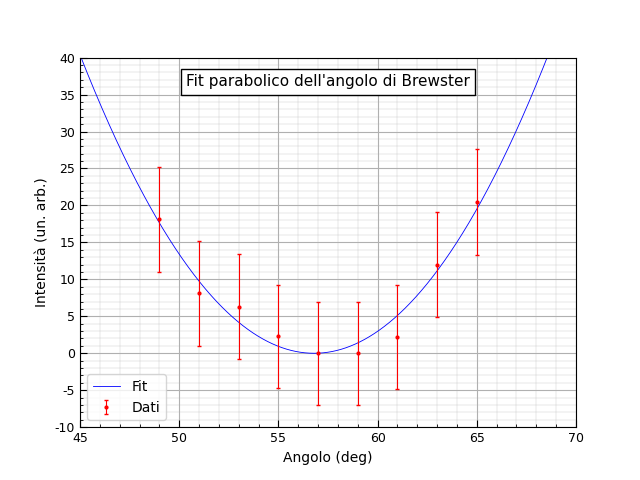
\includegraphics[width=7cm]{./graphs/brewsters-angle.png}
    \caption{\emph{Fit parabolico dell'angolo di brewster.}}
    \label{fig:brewsters-angle}
  \end{figure}
  \begin{table}[ht]
    \centering
    \begin{tabular}[t]{cc}
      \toprule
      Parametro &Valore ottenuto\\
      \midrule
      $a$ &$0.29 \pm 0.02 (un. arb.)$ \\
      $\theta_B$ &$56.8^\circ \pm 0.2^\circ$ \\
      \bottomrule
      \end{tabular}
    \caption{
      Risultati numerici del \emph{fit} parabolico per determinare l'angolo di Brewster.
    }
    \label{tab:fit-brewster}
  \end{table}
\endinput



